\section{Conclusion}
\begin{wrapfigure}{r}{0.5\linewidth}
    \vspace{-2.5mm}
    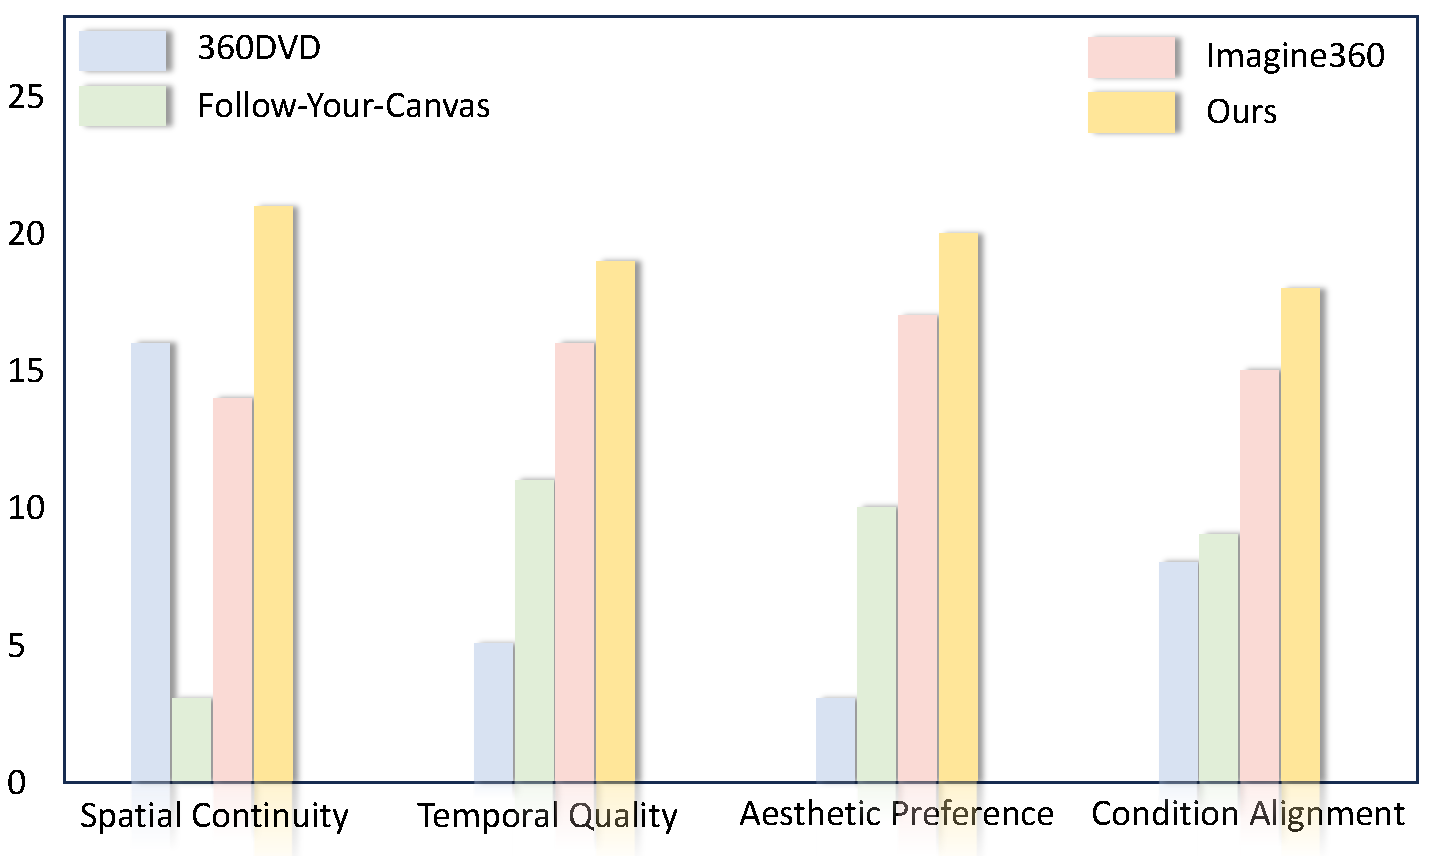
\includegraphics[width=0.9\linewidth]{figs/user.pdf}
    \caption{\textbf{User studies.} We ask participants to vote on the videos generated by four methods based on four dimensions, and our approach receives the most votes.}
     % \vspace{-10.0mm}
    \label{fig:user}
\end{wrapfigure}
In this work, we present ViewPoint, a novel framework for representing and generating panoramic videos leveraging modern generative models. 
%
Specifically, we design a novel representation distinct from traditional panoramic image and video representations, which has the advantage of good spatial continuity and temporal consistency.
%
Through our proposed Pano-Perspective attention mechanism, the pretrained model perceives the global spatial structure information of panoramic videos while modeling fine-grained visual features, effectively improving the quality of the generated videos.
%
To further enhance spatial consistency, we propose an overlapping gradient fusion mechanism that fully utilizes the spatial continuity of each subregion, thereby improving the spatial quality of panoramic videos.
%
Extensive qualitative and quantitative experiments, as well as user studies, demonstrate the effectiveness of our method, and we believe ViewPoint can provide valuable insights for the omnidirectional vision community.